\newpage
\section{State of the art}

% Reading list:
% 	- Pitfalls
% 	- Wu
% 	- Powerful
% 	- Hamilton repr learn
% 	- Hamilton  and 
% 	- GGNN

% ML in graphs intro 
This section is a compilation of several sources that survey the most recent Graph Neural Network advances as well as giving detailed information on their internals. Parts of the text are extracted from the research papers and surveys that follow:
\begin{itemize}
	\item Hamilton et al., Representation Learning on Graphs: Methods and Applications \cite{hamilton} %Hamilton
	\item Xu et al., How Powerful are Graph Neural Networks? \cite{powerful}%strengths
	\item Wu et al., A comprehensive Survey on Graph Neural Networks \cite{wu}%Wu 
	\item Kipf et al., Semi-supervised classification with Graph Convolutional Networks \cite{gcn} %Tkipf
	\item Li et al., Gated graph sequence neural networks \cite{ggnn} %gated graph neural network
\end{itemize}


Many data can be represented as a graph, a data structure employed often in fields like biochemistry, social networks, recommender systems and even computer program analysis. Many machine learning applications are created to make predictions using graph-structured data. The way to incorporate the information from graph-structured data as an input to a machine learning model is not straightforward. The fact that graph-structure data is high-dimensional and non-Euclidean are the main barriers for creating a unified and general way to use it as an input to a model. Graph data is irregular, with variable size and variable number of neighbors. Many approaches to transform graph data into usable features for machine learning models exist by using summary graph statistics, kernel functions, or hand-engineered features. Those approaches lack the flexibility to adapt during the learning process.


% Graph Neural Network quick definition (Hamilton, Wu, GGNN, Hamilton, Powerful, PItfalls)
% 	Graph/Subgraph/Node representation idea -> low dimensional embedding (Hamilton)

The idea behind graph neural networks is to learn a mapping that embeds nodes, or entire subgraphs, as points in a low-dimensional vector space $R^d$. The goal is to optimize this mapping so that geometric relationships in the embedding space reflect the structure of the original graph. Previous approaches to learn on graphs used this approach as a preprocessing step, with fixed and/or hand engineered parameters. The graph neural networks treat this representation learning task as a machine learning task itself, using a data-driven approach to learn the embeddings that encode the desired graph structure.

This section will present the main advances in graph neural networks, showing the techniques for representing nodes and entire subgraphs.

\subsection{Notation}

% 	Graph definition (Wu)
\textbf{Definition of a Graph:} A graph is defined as $G = (V,E,A)$ where $V$ is the set of nodes, $E$ is the set of edges and $A$ is the adjacency matrix. In a graph, let $ v_{i} \in V $ denote a node and $ e_{i,j} = (vi, vj) \in E $ denote an edge. The adjacency matrix A is a N x N matrix with $N = |V|$ where $A_{i,j} = w_{i,j} > 0$ if $e_{i,j} \in E$ and $A_{i,j}=0$ if $e_{i,j} \notin E$. The degree of a node is the number of edges connected to it, formally defined as $ degree(v_i) = \sum A_{i,:}$

A graph can be associated with node attributes X, where $X \in R^{N \times D}$ is a feature matrix with $X_i \in R^{D}$ representing the feature vector of node $v_i$. %In the case of $D = 1$, we replace $x \in R^N$ with X to denote the feature vector of the graph.

\textbf{Definition of a directed graph:} A directed graph is a graph with all edges pointing from one node to another. For a directed graph, $ A_{i,j} \neq A_{j,i} $. An undirected graph is a graph where all edges are bidirectional. For an undirected graph, $A_{i,j} = A_{j,i}$.


% 	Euclidean space definition (Wu, Powerful,pitfalls)
\textbf{Euclidean space:}  a space in any finite number of dimensions, in which points are designated by coordinates (one for each dimension) and the distance between two points is given by a distance formula.  A distance $d$ is defined as a function, let $x,y \in \mathbb{R}^p$:
$$d:\mathbb{R}^{2p} \to \mathbb{R}_{+} \begin{cases}

d(x,y)>0 & \forall x \neq y \\
d(x,y)=0 & iff \quad x=y \\
d(x,y) \leq d(x,z)+d(z,y) & \forall x,y,z

\end{cases}$$

An Euclidean distance $d$ between two points x and y is defined as $d^2(x,y)=(x-y)^T\matchcal{A}(x -y)$ where $\mathcal{A}$ is a positive definite matrix, called a metric.

% 	Non-Euclidean space definition (powerful, pitfalls)
Graph-structured data is considered to be non Euclidean. There's not a clear definition of the norm of a vector representing a node in the space defined by the graph itself. Consequently, the distance between two nodes has to be defined on some other criteria. Usually the distance between two nodes is computed as the number of nodes that exist in the shortest path following edges between the node at the origin and the node at the destination. 
%Second, the distance between nodes, when computed that way, does not fulfill the triangle inequality (3rd condition in the previous definition). 
Moreover, the similarity between nodes, as computed based on the node's attributes, does not need to comply with node distances (as defined by previous sentence ).


\subsection{Original model}

%First Papers, 2005 and 2009, small summary (Wu, Pitfalls)
%	convergence methods
%		- propagation of neighbor information

The idea of a graph neural network was first presented by Gori et al.(2005) \cite{gori} and then developed by Scarselli et al. (2009) \cite{scarcelli}. Good and generic definitions of the process of training a Graph Neural Network are explained at \cite{hamilton} and \cite{powerful}. They are summarized in the following paragraphs. 

% generalised definition (Powerful)
\textbf{Graph Neural Networks:} GNNs use the graph structure and node features $X_v$ for $v \in V$ to learn a representation vector of a node, $h_v$, or the entire graph $h_{G}$. Modern GNNs follow a neighborhood aggregation strategy, where they iteratively update the representation of a node by aggregating representations of its neighbors. After $k$ iterations of aggregation, a node's representation captures the structural information within it's $k$-hop network neighborhood. Formally, the $k$-th layer of a GNN is:
$$ a_v^{(k)} = AGGREGATE^{(k)}(\{ h_u^{(k-1)} : u \in N(v) \}) ,$$ 
$$ h_v^{(k)} = COMBINE^{(k)}(h_v^{(k-1)}, a_v^{(k)}),$$

where $h_v(k)$ is the feature vector of node $v$ at the $k$-th iteration/layer. The initialization consists in $h_v^{(0)} = X_v$, and $N(v)$ is a set of nodes adjacent to $v$. 
The iterative aggregation process is computationally intensive. Modern implementations try to speed up this convergence process, for example by limiting the number of iterations or by using random walks for processing the neighborhood.  To ensure convergence, the recurrent function (the composition of $COMBINE$ and $AGGREGATE$) must be a contraction mapping. A contraction map shrinks the distance between two points after mapping. GNN use the Almeida-Pineda algorithm \cite{AlmeidaPineda} to train the model. The core idea is to run the propagation process to reach a convergence point and then perform the backward procedure given the converged solution.

% 2 tasks
There are two types of tasks, where GNNs are used: node classification/regression and graph classification/regression.  Node classification or regression is when each node $v \in V$ has an associated label or target value $y_v$ and the goal is to learn a representation vector $h_v$ of $v$ such that $v$'s label or target values can be predicted as $y_v=f(h_v)$. Graph classification or regression is when given a set of graphs $\{ G1, ..., G_N\}$ and their labels or target values $\{y_1,...,y_N\}$ the goal is to learn a representation vector $h_G$ that helps to predict the label or target value of the entire graph $y_G=g(h_G)$.

For node classification/regression, the node representation $h_v^{(K)}$ of the final iteration is used for prediction. For graph classification/regression, the READOUT function aggregates node features from the final iteration to obtain the entire graph's representation $h_G$:
$$h_G = READOUT(\{h_v^{(K)} | v \in G\})$$
The READOUT function can be a simple permutation invariant function such as a summation or a more sophisticated graph-level pooling function.

The choice of $AGGREGATE^{(k)}(\cdot)$ and $COMBINE^{(k)}(\cdot)$ is crucial. In the next subsection the main evolutions of this model is explained. The main idea is what choices of $AGGREGATE^{(k)}(\cdot)$ and $COMBINE^{(k)}(\cdot)$  have been used for those state-of-the-art models. 


% slidesCambdribe kipf visual plot of the GNN
\begin{figure}[H]
\centering
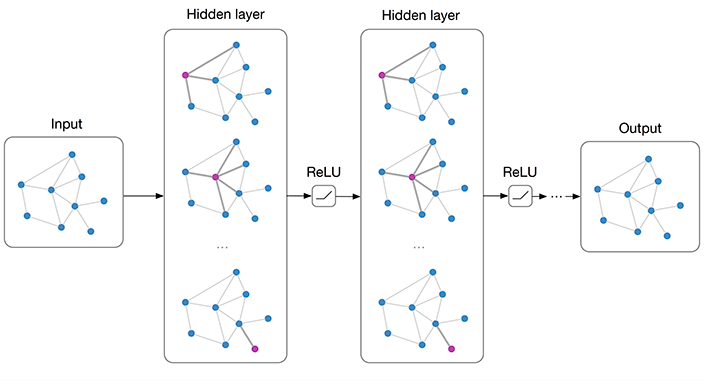
\includegraphics[scale=0.45]{./img/kipf-2.png}\\[2cm] 
\caption{Graph Neural Network architecture (from  Thomas Kipf et al. 2016 \cite{gcn}) }\label{fig:GNN_schema}
\end{figure}

The figure \ref{fig:GNN_schema} shows an example of a 2 layer Graph Neural Network embedding. In each "Hidden layer" of the figure, the model is performing the aggregation and the combination (with readout if needed) phase before producing its output.
 
% comment (review and remove redundancy) FOR INTRO

% It follows a recursive neighborhood aggregation framework (also called message passing), where the representation vector of a node is computed by recursively aggregating and transforming feature vectors of its neighboring nodes. After k iterations, a node is represented by its transformed feature vector, which captures the structural information within the node's k-hop network neighborhood. This approach works when the learning task requires to represent each node of the graph, for example for node attribute regression or node classification. When the learning task requires to compute representations at the graph or subgraph level, pooling mechanisms like addition or other aggregations of all the nodes of the (sub)graph are used. 


% In these publications about graph neural networks, they implement models for learning a node's representation by propagating neighbor information in an iterative manner until convergence in all nodes is reached. This process is computationally intensive, modern implementations try to speed up this convergence process, for example by limiting the number of iterations or by using random walks for processing the neighborhood.




\subsection{Advanced models} 





% spatial versus spectral methods----------------(Wu)
Early models try to learn a node's representation by propagating neighbor information in an iterative manner until convergence in all nodes is reached. This process is computationally intensive and so recently there have been several publications that try to make this process less costly. A large number of methods apply the characteristics of convolutional networks in the computer vision domain to graph data. They are called Graph Convolutional Networks (GCN).

\textbf{Graph Convolutional network:}


% Spectral graph theory approaches (Wu)%(Tkipf)
% Spatial based methods (Wu)
% GNN types overview: (-> Wu taxonomy of GNNs p4)
%   adapt it to what has already been written 

%   GNN (recurrent spatial gcns)
% 		-> adapt

% 	GCN (Hamilton, Kipf)
%	 	-> adapt


%  spectral based--------
The first GCN model is presented in Bruna et al.(2013) \cite{bruna} which develops a variant of graph convolution based on spectral graph theory. There have been several other publications on spectral-based graph convolutional networks \cite{defferrard2016convolutional}.  Spectral methods define graph convolutions by introducing filters from the perspective of graph signal processing, where the graph convolution operation is interpreted as removing noise from graph signals. They rely on the eigen-decomposition of the Laplacian matrix. This has the drawback that any perturbation  of a graph results in a change of eigen basis, and the learned filters are domain dependent so they can't be applied to a graph with a different structure. 


% spatial based-------------
There is another kind of convolutional approach for graphs, called spatial-based graph convolutional networks, see \cite{graphsage} and \cite{geometricdl}. They define graph convolution based on a node's spatial relations. These methods directly perform the convolution in the graph domain by aggregating the neighbor nodes  information. The spatial-based graph convolution takes the aggregation of a node and its neighbors to get a new representation for it. A common practice is to stack multiple graph convolution layers together.


% comparison spatial vs spectral -------------(Wu)
In terms of scalablity and parallelization, the spectral methods  cost increments exponentially with the size of the graph but it needs the whole graph in memory. So these methods are not suitable for large scale data or parallelized architectures. However, spatial methods perform the convolution in the graph domain via aggregating the neighbors attributes so they can handle large graphs. The computation can be performed on batches of nodes instead of the whole graph. Sampling techniques can also be used when the number of neighbors becomes prohibitive.

In terms of generalization of the models, the spectral-based models assume a fixed graph and are not good at generalizing to unseen graphs. Spatial-methods don't have this constraint as their convolution is performed locally and the weights used in the convolution can be shared across different locations.

Finally, spectral methods are limited to work on undirected graphs whereas spatial methods can deal with multi-source inputs and directed graphs by modifying the aggregation function. Spatial-based models are attracting more attention on the scientific comunity than spectral-based models.



% Spatial GCN definiton -----------------------
% (Kipf web page: Weisfeiler Lehman  and GCN comparison)

Let's see how the spatial-based graph convolutional network implements the algorithm that will iteratively generate a representation of the nodes. This algorithm depends on weights, also called coefficients, that will be later updated with stochastic gradient descent or equivalent algorithms. These updating mechanism allows for training an end to end model that contains the representation of the graph generation(the embedding) as well as the subsequent layers that will use the embedding as an input for their classification or regression task.

The previous subsection showed that the updating of a node state (value of its attributes), can be formalized as a function of the node states and the aggregation of the neighbor nodes states:

 $$ h_v^{(k)} = COMBINE^{(k)}(h_v^{(k-1)}, a_v^{(k)})$$,

where $a_v^{(k)}$ is the aggregation of the neighborhood. This same concept can be expressed in matrix notation with the adjacency matrix and matrix of weights in the following equation:


$$H^{(k)} = f(H^{(k-1)},A) =  \sigma(AH^{(k-1)}W^{(k-1)}),$$

where $W^{(k)}$ is a weight matrix for the l-th neural network layer and $\sigma(·)$ is a non-linear activation function like ReLU. Some additional constraints must be imposed on the adjacency matrix A. First, it must be added to the identity I, in order to create self-loops and allow the node attributes to be counted in the updating. Second, A must be normalized.

This functions is implementing the Weisfeiler-Lehman algorithm on graphs, which is used to detect isomorphisms. It assigns a unique set of features for each node that uniquely describes its role in the graph. It works as follows:

For all nodes $v_i \in G$:
\begin{itemize}
\item Get features $\{ h_v_j \}$ of neighboring nodes $\{ v_j \}$
\item Update node feature $h_{v_i}$ = $hash(\sum_j h_v_j)$, where $hash(\cdot)$ is an injective hash function.
\item Repeat for k steps until convergence.
\end{itemize}

Variations of this idea conform the foundations of the more advanced Graph Neural Network models seen in this subsection, the Graph Convolutional Network and its variants, like GraphSage or the Graph Isomorphism Network called GIN.

%GCN definition (kipf web, slides-cambridge)------------

The Graph Convolutional Network model uses filter parameters $W^{(k)}$ that are shared over all locations in the graph:

$$ h^{(k)}_{v_i} = \sigma(\sum_j \frac{1}{c_{ij}}h^{(k-1)}_{v_j}W^{(k-1)})$$

where j indexes the neighboring nodes of $v_i$, and $c_{ij}$ is a normalization constant for the edge $(v_i,v_j)$. This version is a differentiable and parameterized variant of the hash function used in the original Weisfeiler-Legman algorithm. With proper initialization (Glorot) this update rule is stable.



% Powerful paper definition of the aggreation and combine
% In Graph Convolutional Networks (GCN) \cite{gcn}, the AGGREGATE is formulated as:
% $$a_v^{(k)} = MEAN(\{ ReLU(W \cdot h_u^{(k-1)}), \forall u \in N(u) \}) $$
% Where W is a learnable matrix. In GCN, the COMBINE step is omitted and the model simply aggregates node $v$ with its neighbors as $h_v^{(k)} = AGGREGATE(\{ h_v^{(k-1)}, h_u^{(k-1)}: u \in N(v) \})$.


% Graph pooling modules-------------------

When the model is trained to perform classification on the whole graph or a subgraph, a graph pooling module must be used. GCNs that use pooling modules are as powerful as the Weisfeiler-Legman test in distinguishing graph structures. Similar with the pooling layer of CNNs, graph pooling module could easily reduce the variance and computation complexity by down-sampling in between convolutional layers. Mean, max and sum pooling are the most common way to implement them.


The remaining part of the subsection will present evolutions of the GCN model that are most commonly known.

%   MPNN (composition based spatial gcns)
\textbf{Message Passing Neural Networks (MPNN):} The MPNN model generalizes several existing graph convolution networks into a unified framework named Message Passing Neural Network. It consists of two phases, the message passing phase and the readout phase. The message passing phase actually runs T-step spatial-based graph convolutions. The graph convolution operation is defined through a message function $M_t(\cdot)$ and an updating function $U_t(\cdot)$ according to 

$$ h_v^t = U_t(h_v^{(t-1)}, \sum_{w \in N(v)} M_t(h_v^{t-1}, h_w^{t-1}, e_{vw}))$$

The readout phase is actually a pooling operation which produces a representation of the entire graph based on hidden representations of each individual node. It is defined as 

$$ y' = R(h_v^T|v \in G) $$

Through the output function $R(\cdot)$, the final representation $y'$ is used to perform graph-level prediction tasks. The authors \cite{mpnn} state that several other graph convolution networks fall into their framework by assuming different forms of $U_t(\cdot)$ and $M_t(·)$.

% GraphSage----------------(Hamilton )

\textbf{GraphSage:} It introduces in \cite{graphsage} the notion of the aggregation function to define the graph convolution. The aggregation function essentially assembles a node's neighborhood information. It must be invariant to permutations of node orderings such as mean, sum and max. The graph convolution operation is defined as, 

$$ h_v^t = \sigma(W^t \cdot aggregate_k(h_v^{t-1}, \{h_u^{k-1}, \forall u \in N(v)\}))$$

Instead of updating states over all nodes, GraphSave proposed a batch-training algorithm, which improves scalability for large graphs. The learning process of GraphSage consists of three steps. First, it samples a node's local k-hop neighborhood with fixed-size. Second, it derives the central node's final state by aggregating its neighbors feature information. Finally, it uses the central node's final state to make predictions and backpropagate errors. Assuming the number of neighbors to be sampled at the $t^{th}$ hop is $s_t$, the time complexity of GraphSage in one batch is $O(\prod_{t=1}^{T}s_t)$. Therefore the computation cost increases exponentially with the increase of $t$. This prevents GraphSage from having a deep architecture. However, in practice, the authors find that with t=2 GraphSage already achieves high performance.

% In the pooling variant of GraphSAGE \cite{graphsage}, the mean operation is replaced by an element-wise max-pooling. The COMBINE step could be a concatenation followed by a linear mapping $W \cdot [h_v^{(k-1)} | a_v^{(k)}]$ as in GraphSAGE.
% % Transductive vs inductive approaches (GraphSage)



%  GGNN
\textbf{Gated Graph Neural Networks (GGNN):} also known as GGNN, this kind of GNN employ the gated recurrent units (GRU) \cite{GRU} as the recurrent function, reducing the recurrence to a fixed number of steps. The spatial graph convolution of GGNNs is defined as 

$$ h_v^t = GRU(h_v^{(t-1)}, \sum_{u \in N(v)} Wh_u^t) $$

For updating of the weights, the GGNNs use back-propagation through time (BPTT) to learn the parameters. The advantage is that it no longer needs to constrain parameters to ensure convergence. However, the downside of training by BPTT is that it sacrifices efficiency both in time and memory. This  is especially problematic for large graphs, as GGNNs need to run the recurrent function multiple times over all nodes, requiring intermediate states of all nodes to be stored in memory.


% Other types (Wu) -> quickly summarize them

Other types of GGNs are the Graph attention Networks, Graph Auto-encoders, Graph Generative Networks and Graph Spatio-temporal Networks.

\textbf{Graph Attention Networks} are similar to GCNs and seek an aggregation function to fuse the neighboring nodes, random walks, and candidate models in graphs to learn a new representation. The key difference is that graph attention networks employ attention mechanisms which assign larger weights to the more important nodes, walks, or models. The attention weight is learned together with neural network parameters within an end-to-end framework.

\textbf{Graph Auto-encoders} are unsupervised learning frameworks which aim to learn a low dimensional node vectors via an encoder, and then reconstruct the graph data via a decoder. Graph autoencoders are a popular approach to learn the graph embedding, for both plain graphs without attributed information as well as attributed graphs. For plain graphs, many algorithms directly pre-process the adjacency matrix, by either constructing a new matrix (i.e., point-wise mutual information matrix) with rich information, or feeding the adjacency matrix to an autoencoder model and capturing both first order and second order information. For attributed graphs, graph autoencoder models tend to employ GCN as a building
block for the encoder and reconstruct the structure information via a link prediction decoder.

\textbf{Graph Generative Networks} aim to generate plausible structures from data. Generating graphs given a graph empirical distribution is fundamentally challenging, mainly because graphs are complex data structures. To address this problem, researchers have explored to factor the generation process as forming nodes and edges alternatively, to employ generative adversarial training. One promising application domain of graph generative networks is chemical compound synthesis. In a chemical graph, atoms are treated as nodes and chemical bonds are treated as edges. The task is to discover new synthesizable molecules which possess certain chemical and physical properties. 

\textbf{Graph Spatial-temporal Networks} aim to learn unseen patterns from spatial-temporal graphs, which are increasingly important in many applications such as traffic forecasting and human activity prediction. For instance, the underlying road traffic network is a natural graph where each key location is a node whose traffic data is continuously monitored. By developing effective graph spatial temporal network models, we can accurately predict the traffic status over the whole traffic system. The key idea of graph spatial-temporal networks is to consider spatial dependency and temporal dependency at the same time. Many current approaches apply GCNs to capture the dependency together with some RNN or CNN to model the temporal dependency.


\subsection{Alternatives to Graph Neural Networks}


% Theoretic alternatives to GNN (Hamilton, GGNN)
% 	- summary graph statistics
% 	- kernel functions (Hamilton)
% 	- random walks , and matrix factorization
% 		- factorizaion -based embeding (Hamilton)
Alternatives to Graph Neural Networks existed long before their first appearance: summary graph statistics, kernel functions and network embeddings (matrix factorization and random walks).

Summary statistics aim to capture very specific features of the whole graph, hoping that they will allow the model to discriminate or predict values. The most common ones are the average node degree, the clustering coefficient as well as the assortativity. They usually lack a lot of representation flexibility and fail to correctly capture aspects of the graph structure that are not reflected by those summary statistics


Kernel functions allow to capture much more signal from the graph structure, and then can be used to build powerful classification or regression algorithms. They are also used in unsupervised learning approaches. The drawback from kernels is that they are not suitable for large scale graphs, as they need to have the whole graph in memory.

% Wu survey p2 network embeddings description
 
Network embeddings aim to represent network vertices's into a low-dimensional vector space, by preserving both network topology structure and node content information. This embedding can be used in any downstream shallow machine learning algorithm, such as classification, regression, or clustering, in the same way that the output of a GGN is. Many network embedding algorithms are typically unsupervised algorithms and they can be broadly classified into three groups: matrix factorization \cite{38}, random walks \cite{40}, and deep learning approaches.\\
\\

% 	Most prominent matrix factorization methods ?
% 	Most prominent distance methods (and combinations) ?



% Observations on current research
% 	- subsequent research papers using the same datasets and training/val/test splits -> they overfit to the dataset and defeat the purpose of generalization.







\subsection{Applications of Graph neural Networks}


%--ML--tasks
Finally, this section presents the most important applications of Graph Neural Networks and its variants. The applications in several specific domains all fall under the following list of machine learning tasks to which GNNs are showing good results:
\begin{itemize}
	\item node classification/regression
	\item graph classification/regression
	\item graph generation
	\item graph visualization
	\item node clustering
	\item link prediction
	\item graph partition
\end{itemize}


% 	- Computer vision
\textbf{Computer Vision:} in this domain, research has been done to perform scene graph generation, point cloud classification and segmentation, and action recognition. In scene graph generation, semantic relationships between objects facilitate the understanding of the semantic meaning behind a visual scene. Given an image, scene graph generation models detect and recognize objects and predict semantic relationships between pairs of objects \cite{121}. In point clouds classification and segmentation, \cite{125}, the task is to identify the objects depicted by point clouds, by using graph convolution networks to explore the topological structure. In action recognition, persons recognized in an image(or video) have their joints detected and their connections form a graph that can be analyzed with spatial-temporal neural networks to classify human actions.

% 	- recommender systems (GNN Hamilton repr learning,)
\textbf{Recommender Systems:} graph based recommender systems take items and users as nodes. By leveraging the relations between items and items, users and users, users and items, as well as content information, graph-based recommender systems are able to produce high-quality recommendations. The key to a recommender system is to score the importance of an item to an user. As a result, it can be cast as a link prediction problem. The goal is to predict the missing links between users and items(\cite{9},\cite{10},\cite{11}).

% 	- Chemistry
\textbf{Biochemistry:} graph neural networks are used to classify the molecules structure. Nodes represent atoms and edges represent chemical bonds. Node classification, graph classification and graph generation are the three main tasks. Examples include learning molecular fingerprints \cite{52}, predict molecular properties \cite{mpnn} and to synthesize chemical compounds \cite{65}


\textbf{Communications Network modeling:} Communication networks rely on routing and path optimization to ensure good level of service. Nowadays network operators lack efficient network models able to make accurate predictions of relevant end-to-end Key Performance Indicators (KPI) such as delay or jitter at limited cost. Analytic models and packet-level simulations have been used to produce KPI's but at a high cost. A graph neural network model, RouteNet \cite{rusek2019unveiling}, has been proposed as an efficient solution to produce estimations of delay and jitter with similar accuracy as packet-level network simulators.


\textbf{Program verification:} is another fruitful domain where Graph Neural Networks are showing their potential (\cite{ggnn}, \cite{139} and \cite{code2vec}). Instructions follow a sequence of execution with loops, branches and calls to other instructions. This kind of modeling of the code allows for verification of correct variable usage (avoid usage after free of a memory buffer), variable name guessing and function renaming for correct understanding of code functionality. Gated Graph Sequence Neural Network \cite{ggnn}, known as GGNN, are Graph Neural Networks that make use of gated recurrent units and modern optimization techniques that can output sequences. They poses a favorable inductive bias relative to purely sequence-based models like LSTMs, when the problem is graph-structured. They achieve state-of-the-art performance on program verification applied to memory safety, to map the state of the memory as a set of input graphs into a logical description of the data structures. For example this can be used to verify that there are no null pointer dereferences in a program. In \cite{139}, the authors use graphs to represent both the syntactic and semantic structure of code and use graph-based deep learning methods to learn to reason over program structures. They apply a modified version of GGNN to the task of VarNaming (predicting the name of a variable given its usage) and VarMisuse (reason about selecting the correct variable in a given program location). Finally, an approach to predicting names for entire functions or subroutines is shown in \cite{code2vec}, where no Graph Neural Network approach has been used, instead an embedding is generated from Abstract syntax trees. It is used for snippets of code to predict semantic properties. We believe that Graph Neural Networks have great potential to achieve state of the art performance.


% Girvan-Newmann algorithm
% 	definition
% 	history
% 	usage
\textbf{Social Network analysis:} With the rapid expansion of the web, the last years have witnessed large adoption of social networks as one of the main ways to interact with people. Graph Neural Networks have many direct applications in social network analysis as friend or link prediction \cite{liben2007link}, community detection \cite{gcn} and many more as can be seen in \cite{hamilton} and \cite{fey2019fast}. One of the main tasks in social network analysis is the process of discovering communities, known as community detection. The Girvan-Newman algorithm \cite{girvan2002community} is a clustering based approach to perform community detection, and is considered one of the most powerful algorithms. It proposed a divisive algorithm based on edge-betweenness for a graph with undirected and unweighted edges. The algorithm focused on edges that are most "between" the communities and communities are constructed progressively by removing these edges from the original graph.The worst-case for time complexity of the edge-betweenness algorithm is $O(m^2n)$ and is $O(n^3)$ for sparse graphs, with $m$ being the number of edges and $n$ the number of vertices's. Its downside is that it is very time consuming which makes it not suitable for applying it to modern social networks. As surveyed by \cite{Bedi}, many authors have worked to improve it, reduce the computational complexity or extract useful concepts from it (see \cite{Radicchi} and \cite{Rattigan}, \cite{Chen}, \cite{Newman2} ). 



%21, 29,  22,  33




